% Format verslag in LaTeX maken.
% Lars Aalsma, Tutor Natuur- en Sterrenkunde 2014-2015
% & Ramon Creyghton, tutor Natuur- en Sterrenkunde 2014-2016.
% & David Fokkema, staflid natuurkundepracticum, september 2017.
%
% Dit document mag naar eigen inzicht aangepast en verspreid worden.
% Her en der in dit document staan opmaak-opties en packages opgenomen, die afhankelijk van je voorkeuren kunnen worden aan- of uitgezet. Het is aan te raden je te verdiepen in de werking van deze opties (ze googlen is een start) voor je ze gebruikt.

\documentclass[11pt,a4paper]{article}

\usepackage{fouriernc}        % Dit package kiest het lettertype. Laat dit weg voor standaard Computer Modern.
\usepackage[utf8]{inputenc}   % Je kunt gewóón accenten typen, als je wilt
\usepackage[T1]{fontenc}      % Nodig om de accenten ook ín de pdf te krijgen
\usepackage[dutch]{babel}     % Figuur i.p.v. Figure, en NL afbrekingen
\usepackage{graphicx}         % Voor \includegraphics om figuren in te voegen
\usepackage{amssymb}          % Voor extra symbolen
\usepackage{amsmath}          % Voor extra ondersteuning bij vergelijkingen (zie documentatie)
\usepackage{natbib}           % Voor auteur-jaar citatie.
\usepackage{a4wide}           % Past marges aan voor A4.
\usepackage[small]{caption}   % Voor bijschriften met een iets kleinere lettergrootte dan de hoofdtekst.
\usepackage{url}              % Voor het beter weergeven van url's (lang, of met speciale tekens)
\usepackage{booktabs}         % Voor professionele tabellen
\usepackage[output-decimal-marker={,},list-final-separator={ en }]{siunitx}          % Voor het typesetten en uitlijnen van getallen en eenheden, zie documentatie
\usepackage[pdfusetitle]{hyperref}  % Voor handige links in je PDF. B.v. urls, referenties, etc.
\usepackage[version=4]{mhchem}
\usepackage{physics}


\linespread{1.3}              % Iets grotere regelafstand: fijn voor degene die het nakijkt.

% \renewcommand{\arraystretch}{1.5}   % Om rijen in tabellen wat ruimer rond de tekst te maken.

%% DOCUMENT PROPERTIES % vul in
\title{Analyserapport voor de bepaling van de halfwaardetijd van kalium-40} % Vul in.
\date{\today}

\begin{document}

%% BEGIN TITELPAGINA
\begin{titlepage}
\maketitle
\thispagestyle{empty} % geen paginanummer op de titelpagina

\vfill

% Een samenvatting kun je opnemen op je titelpagina met het commando hieronder. 
%\abstract{\small Lorem ipsum dolor sit amet, consectetur adipiscing elit. Ut tempor ullamcorper sapien, quis lacinia nibh pellentesque vel. Sed ultrices nunc vitae magna pulvinar ac posuere velit bibendum. Nunc placerat ornare libero nec viverra. Nulla ullamcorper diam orci, sit amet scelerisque nisl. Nam sapien felis, auctor vestibulum dignissim nec, egestas eget dolor. \\[2ex]}

 \begin{table}[h]
  \label{tab:credits}
  \begin{tabular}{l l}
   \textsc{Auteur} & Frenk Klein Schiphorst \\
   \textsc{Studentnummer}  & 11866497 \\ % Vul in
   \textsc{Vak} & Natuur- \& Sterrenkunde Practicum 2 \\
   \textsc{Studie} & Natuur- \& Sterrenkunde\\
  \end{tabular}
  \vspace{3ex}
 \end{table}

%De regels hieronder zorgen voor een mooi VU-UvA op je titelpagina. Het bestand logo-combi-vu-uva-nl.png is dan wel noodzakelijk.
%Pro-tip: Bij regelmatig gebruik kan het handig zijn om dit bestand in je 'texmf' folder te zetten (Google is je vriend)
\begin{figure}
  \centering  
  
\includegraphics[width=150mm]{logo-combi-vu-uva-nl}\\   % UvA logo
  \vspace{-13ex}
 \end{figure}

\end{titlepage}
%% EIND TITELPAGINA

\setcounter{page}{2}    % Begin na de titelpagina op pagina 2, dat is iets netter

\suppressfloats[t]      % Nu volgt eigenlijk de eerste pagina van het document. Je wilt dan niet beginnen met een figuur. Dit commando (suppress floats at top of the page) onderdrukt een eventueel figuur en schuift dat naar een andere positie. Dit commando geldt alleen voor de *huidige* pagina.

%%BEGIN VAN DE INHOUD VAN HET DOCUMENT

\section{Inleiding}
In dit analyserapport wordt de bepaling van de halfwaardetijd van kalium-40 gepresenteerd. De gebruikte meetdata bestond uit metingen van de activiteit van bepaalde hoeveelheden kaliumcarbonaat, \ce{K2CO3}. De metingen zijn gedaan met een Geiger-Muller (GM) telbuis.

\section{IJken GM-buis}

Elke GM-buis heeft een efficiëntie, die staat voor de kans dat een deeltje afkomstig van een bron gemeten wordt. De efficiëntie volgt uit
\begin{equation}
\epsilon = \epsilon_g \epsilon_i
\label{eq:efficientie}
\end{equation}
met $\epsilon_g$ de geometrische efficiëntie en $\epsilon_i$ de intrinsieke efficiëntie. De geometrische efficiëntie hangt af van de opstelling, en staat voor de kans dat een deeltje in de richting van het intreevenster uitgezonden wordt. De intrinsieke efficiëntie hangt af van het soort straling.

De intrinsieke efficiëntie van de gebruikte GM-buis is onbekend. Om deze te bepalen zijn ijkmetingen gedaan met zes andere GM buizen. De ijkbron was een strontium-90 bron met bekende activiteit. Aan de hand van een fit is te bepalen of de zevende GM buis, waarmee de metingen aan het kaliumcarbonaat zijn gedaan, ofwel dezelfde intrinsieke efficiëntie had als de andere zes (optie 1), ofwel een iets andere intrinsieke efficiëntie (optie 2). Optie 1 zou betekenen dat de verschillen in de gemeten deeltjes per GM buis alleen veroorzaakt worden door de fout in de telstatistiek. Als dit niet het geval is, geldt optie 2 en wordt voor de intrinsieke efficiëntie van de zevende buis het gemiddelde van de andere zes genomen.

\subsection{Meetdata}
Met elk van de zes GM-buizen is een ijkmeting gedaan. De ijkbron had een activiteit van 1400 Bq. De bron bevond zich op 15.0 cm van het intreevenster van de GM-buis. Het ronde intreevenster had een diameter van 3.0 cm. Ook is er met elke GM-buis een achtergrondmeting gedaan. Alle metingen duurden 480 s. De resultaten van de metingen staan in tabel \ref{tab:tabel1}. De telstatistiek wordt bepaald door de Poissonverdeling. De fout op de getelde deeltjes worden daarom gegeven door de wortel van het aantal getelde deeltjes zelf.

\begin{table}
\caption{Meetdata van de ijkmetingen. De fouten op de aantallen counts worden gegeven door de wortel van het aantal counts zelf.}
\centering
\resizebox{\textwidth}{!}{\begin{tabular}{SSSSS} % uitlijnen als getal, dus met de komma's b.v. recht onder elkaar.
\toprule
{Nummer GM-buis} & {Aantal counts met bron} & {Fout op aantal counts} & {Achtergrondcounts} & {Fout op achtergrond} \\  % Kop moet tussen {} om uitlijning als getal te voorkomen
\midrule
7	&	1399	&	 37.40 	&	187	&	13.67	\\
9	&	1455	&	 38.14 	&	159	&	12.61	\\
10	&	1421	&	 37.70 	&	212	&	14.56	\\
11	&	1580	&	 39.75 	&	154	&	12.41	\\
13	&	1418	&	 37.66 	&	177	&	13.30	\\
15	&	1589	&	 39.86 	&	183	&	13.53	\\
\bottomrule
\end{tabular}}
\label{tab:tabel1}
\end{table}

\subsection{Uitwerking}
Het aantal counts afkomstig van het strontium is te berekenen door het aantal achtergrondcounts van het totale aantal gemeten counts af te halen. De fout hierop wordt bepaald aan de hand van de algemene formule voor foutenpropagatie:
\begin{equation}
\delta q = \sqrt{\left(\pdv{q}{x}\delta x\right)^2 + ... + \left(\pdv{q}{z}\delta z\right)^2}
\label{eq:foutenpropagatie}
\end{equation}

Omschrijven van vergelijking \ref{eq:foutenpropagatie} geeft voor de fout op het aantal counts afkomstig van de strontium-bron:
\begin{equation}
\delta \text{strontium} = \sqrt{\left(\delta \text{counts}\right)^2 + \left(\delta \text{achtergrond}\right)^2}
\label{eq:fout_strontium}
\end{equation}

De totale hoeveelheid deeltjes afkomstig van de strontium-bron is te berekenen. Per vervalsreactie van strontium-90 komen er twee $\beta^-$-deeltjes vrij. Met een activiteit van 1400 Bq en een meetduur van 480 s volgt hieruit voor het totale aantal deeltjes:
\begin{equation}
\text{aantal deeltjes} = 1400 * 2 * 480 = 1.334.000
\label{eq:aantal_deeltjes_ijkbron}
\end{equation}

Op zowel de activiteit van de bron als de duur van de meting zit een fout van 1. Hieruit volgt, via vergelijking \ref{eq:foutenpropagatie}, voor de fout op het totale aantal deeltjes:
\begin{equation}
\text{fout aantal deeltjes} = \sqrt{\left(960\right)^2 + \left(2800\right)^2} = 2960
\end{equation}

Voor de totale efficiëntie van de gebruikte GM-buizen geldt:
\begin{equation}
\epsilon = \frac{\text{aantal gemeten deeltjes}}{\text{totaal uitgezonden deeltjes}}
\label{eq:efficientie_GM}
\end{equation}
Ook hier zit een fout op, die weer volgt uit vergelijking \ref{eq:foutenpropagatie}. Vervolgens is met de geometrische efficiëntie en vergelijking \ref{eq:efficientie} de intrinsieke efficiëntie van de GM-buizen te bepalen. De geometrische efficiëntie is te berekenen als de verhouding tussen de oppervlakte van het intreevenster van de GM-buizen en de oppervlakte van de bolschil waarover de straling vanaf de ijkbron verdeeld wordt. De formule is:
\begin{equation}
\epsilon_g = \frac{\pi r^2}{4\pi R^2}
\label{eq:geometrisch}
\end{equation}
met $r$ de straal van het intreevenster en $R$ de straal van de bolschil. Uiteraard weer met fout volgens vergelijking \ref{eq:foutenpropagatie}. De straal van het intreevenster is hier 1.5 cm, met een fout van 0.1 cm. De straal van de bolschil is gelijk aan de afstand van de bron tot de detector, 15.0 cm, ook met een fout van 0.1 cm.


%\section{Inleiding}
%
%Lorem ipsum dolor sit amet, consectetur adipiscing elit. Ut tempor ullamcorper sapien, quis lacinia nibh pellentesque vel. Sed ultrices nunc vitae magna pulvinar ac posuere velit bibendum. Nunc placerat ornare libero nec viverra. Nulla ullamcorper diam orci, sit amet scelerisque nisl. Nam sapien felis, auctor vestibulum dignissim nec, egestas eget dolor. Suspendisse iaculis, diam pulvinar luctus iaculis, ipsum nisl consectetur nisi, a lacinia eros lacus vitae dui. In fermentum ante quis ante porttitor congue. Mauris sollicitudin rhoncus dictum. Donec pretium molestie tempus. Integer suscipit egestas erat sit amet volutpat. Nullam et magna risus. Nam vel nisi libero. Duis ultricies ipsum eu lorem congue vestibulum. Aenean ut felis velit, ac lacinia erat. In a dolor dignissim elit faucibus facilisis. Vivamus iaculis ornare lacus, viverra convallis sapien pulvinar vitae.
%
%\section{Figuren en tabellen}
%Een voorbeeld van een figuur is op de volgende pagina gegeven, zie figuur \ref{fig:figuur1}. Figuren staan nóóit in de lopende tekst. Pak een willekeurig artikel en je zult zien dat figuren óf bovenaan een pagina staan, óf onderaan een pagina, óf op een eigen pagina. Nooit in het midden. Probeer dus ook niet met \verb|[h]| o.i.d. de plaatsing van figuren te forceren. Over het algemeen maak je het alleen maar erger.
%
%\begin{figure}  % Forceer je figuur niet naar [h]ere. Dat gebeurt in artikelen ook niet.
%\centering
%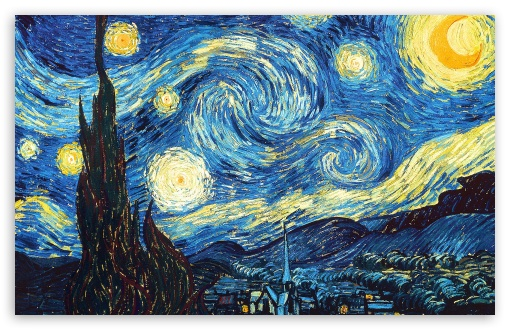
\includegraphics[scale=0.5]{figuur1}
%\caption{Een figuur heeft een onderschrift. Een plaatje trekt al snel je aandacht weg van de hoofdtekst. Zodra je het plaatje snel bekeken hebt, is de natuurlijke neiging om `verder te lezen' en beweegt je aandacht naar onder het plaatje. Als dáár dan een stukje tekst met uitleg staat, wordt het sneller gelezen dan wanneer dat bóven de figuur staat. Blijkt uit onderzoek.}
%\label{fig:figuur1}
%\end{figure}
%
%Een voorbeeld van een tabel is hieronder gegeven, zie tabel \ref{tab:tabel1}.
%
%\begin{table}
%\caption{Een tabel heeft een bovenschrift. Een plaatje of tabel (met veel witruimte eromheen) trekt al snel je aandacht weg van de hoofdtekst. Toch worden je ogen al snel richting de kop getrokken (wat staat er boven de kolommen?) en als dáár dan een stukje tekst met uitleg staat, lees je dat sneller dan wanneer het ónder de tabel staat. Blijkt uit onderzoek.}
%\centering
%\begin{tabular}{SS} % uitlijnen als getal, dus met de komma's b.v. recht onder elkaar.
%\toprule
%{Slingerlengte [\si{\centi\meter}]} & {Slingertijd [\si{\second}]} \\  % Kop moet tussen {} om uitlijning als getal te voorkomen
%\midrule
%5 & 4.5 \\
%10 & 6.3 \\
%15 & 7.8 \\
%20 & 9.0 \\
%25 & 10.0 \\
%\bottomrule
%\end{tabular}
%\label{tab:tabel1}
%\end{table}
%
%\section{Een sectie}
%
%Formules in \LaTeX\ gaan vanzelf al snel goed. Zo krijgt iedere vergelijking automatisch een nummer, dat keurig rechts wordt uitgelijnd. Menig student krijgt dat in Word o.i.d. niet goed voor elkaar. Denk er wel aan formules op te nemen in de lopende tekst.
%\begin{equation}
%  F = ma
%  \label{eq:eerste-wet-newton}
%\end{equation}
%De eerste wet van Newton. Vergelijking \ref{eq:eerste-wet-newton} is níet opgenomen in de lopende tekst, en dat leest dus niet zo lekker door. Je moet jezelf afvragen: kan ik dit verhaal voorlezen? Als je het verhaal goed kunt voorlezen \emph{inclusief} de vergelijking, zonder haperingen, dan staat het goed.
%
%Zo is bijvoorbeeld de trillingstijd van een slinger gegeven door
%\begin{equation}
%  T = 2\pi\sqrt{\frac{l}{g}},
%  \label{eq:trillingstijd-slinger}
%\end{equation}
%met de trillingstijd $T$, de lengte van de slinger $l$ en de valversnelling $g$. Let ook op de komma aan het eind van vergelijking~\ref{eq:trillingstijd-slinger}. Dit stukje tekst kun je vloeiend voorlezen, zonder haperingen. Geef je vergelijkingen ook \emph{namen} om aan te refereren, en geen \emph{nummers}.
%
%Lorem ipsum dolor sit amet, consectetur adipiscing elit. Ut tempor ullamcorper sapien, quis lacinia nibh pellentesque vel. Sed ultrices nunc vitae magna pulvinar ac posuere velit bibendum. Nunc placerat ornare libero nec viverra. Nulla ullamcorper diam orci, sit amet scelerisque nisl. Nam sapien felis, auctor vestibulum dignissim nec, egestas eget dolor. Suspendisse iaculis, diam pulvinar luctus iaculis, ipsum nisl consectetur nisi, a lacinia eros lacus vitae dui. In fermentum ante quis ante porttitor congue. Mauris sollicitudin rhoncus dictum. Donec pretium molestie tempus. Integer suscipit egestas erat sit amet volutpat. Nullam et magna risus. Nam vel nisi libero. Duis ultricies ipsum eu lorem congue vestibulum. Aenean ut felis velit, ac lacinia erat. In a dolor dignissim elit faucibus facilisis. Vivamus iaculis ornare lacus, viverra convallis sapien pulvinar vitae.
%
%\section{Referentie voorbeelden}
%
%\citet{Kachru2003} hebben aangetoond dat de Sitter vacua voorkomen in snaartheorie. Dit werd echter in een latere publicatie tegengesproken \citep{Bena2010}.
%
%%Refereren met LaTeX kan op twee manieren, zie ook Hoofdstuk 5 van de handleiding AVT. Hier voegen we referenties handmatig toe door gebruik te maken van thebibliography, zie de regels hieronder beginnend bij \begin{thebibliography}{}. Elke nieuwe referentie wordt toegevoegd met \bibitem.
%
%%In een \bibitem geeft de tekst tussen de [...] aan hoe de referentie verschijnt in de tekst. Tussen de {...} staat het label waarmee in de tekst naar de referentie kan worden verwezen. Refereren in de tekst wordt gedaan zoals hierboven (met \citet{<label>} en \citep{<label>}).



\end{document}
